\documentclass[xetex,mathserif,serif]{beamer}
\usepackage{polyglossia}
\setdefaultlanguage[babelshorthands=true]{russian}
\usepackage{minted}
\usepackage{tabu}

\useoutertheme{infolines}

\usepackage{fontspec}
\setmainfont{FreeSans}
\newfontfamily{\russianfonttt}{FreeSans}

\usepackage{textpos}
\setlength{\TPHorizModule}{1cm}
\setlength{\TPVertModule}{1cm}

\setbeamertemplate{blocks}[rounded][shadow=false]

\setbeamercolor*{block title alerted}{fg=red!50!black,bg=red!20}
\setbeamercolor*{block body alerted}{fg=black,bg=red!10}

\tabulinesep=1.2mm

\title{Занятие 6: декомпозиция и оценка задач}
\author[Юрий Литвинов]{Юрий Литвинов\\\small{\textcolor{gray}{yurii.litvinov@gmail.com}}}
\date{09.10.2019}

\newcommand{\attribution}[1] {
	\begin{flushright}\begin{scriptsize}\textcolor{gray}{\textcopyright\; #1}\end{scriptsize}\end{flushright}
}

\begin{document}

	\frame{\titlepage}

	\section{WBS}

	\begin{frame}
		\frametitle{Work Breakdown Structure}
		\begin{center}
			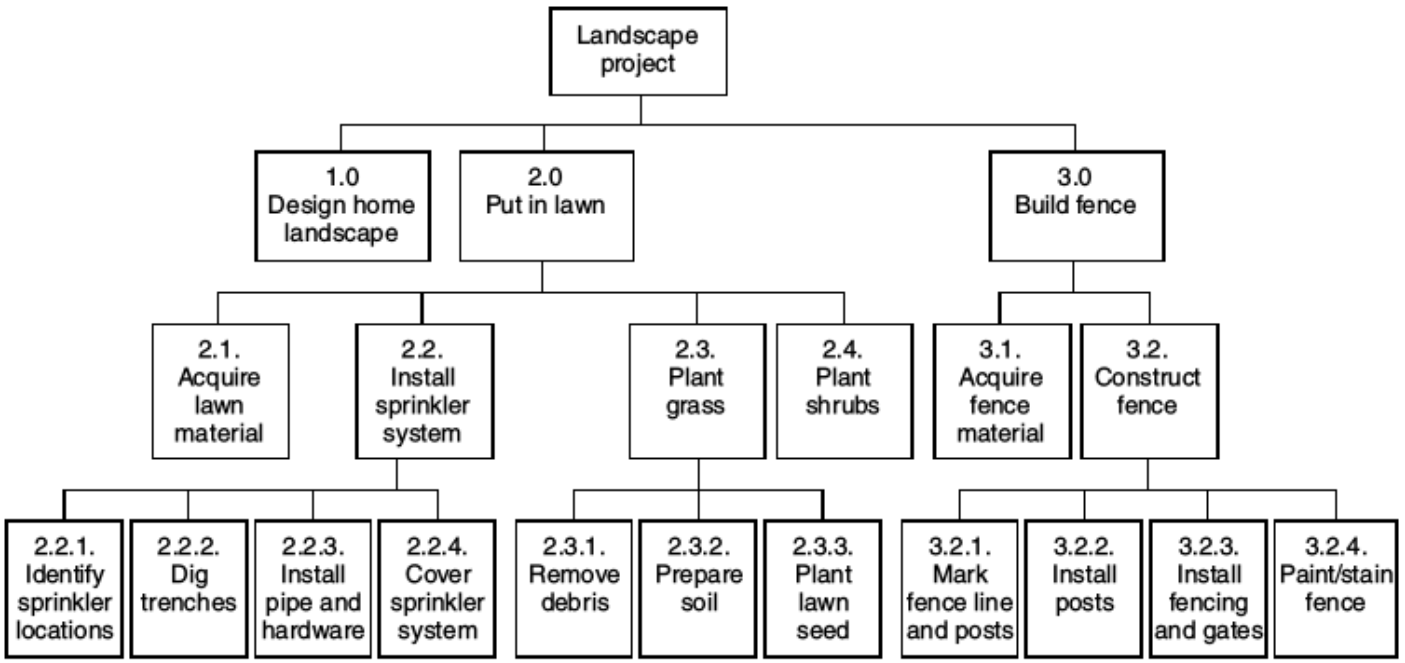
\includegraphics[width=\textwidth]{wbs.png}
		\end{center}
	\end{frame}

	\section{Домашнее задание}
	
	\begin{frame}
		\frametitle{Домашнее задание}
		\framesubtitle{Оценка рисков}
		Написать документ примерно на пару страниц, описывающий риски проекта
		\begin{itemize}
			\item Описание риска
			\item Последствия
			\item Вероятность (низкая/средняя/высокая)
			\item Влияние на проект (низкое/среднее/высокое)
			\item Меры предотвращения
			\item Меры устранения последствий
		\end{itemize}
		Выложить на вики проекта
	\end{frame}

	\section{Задание на пару}

	\begin{frame}
		\frametitle{Задание на пару}
		\begin{itemize}
			\item Выполнить декомпозицию задач проекта
			\item Нарисовать Work Breakdown Structure
			\begin{itemize}
				\item Mind maps
				\item Любой из бесплатных инструментов
			\end{itemize}
			\item Выполнить оценку каждой задачи
			\begin{itemize}
				\item Методом ``снизу вверх''
				\item Методом ``сверху вниз''
			\end{itemize}
			\item Занести задачи в бэклог
		\end{itemize}
	\end{frame}

\end{document}
